% 09_integration.tex
\section{Integration and manufacture}\label{sec:integration}

\subsection{Print geometry}

The printed parts are built from the density field at an iso level of 0.3. The iso surface is smoothed and trimmed to the design envelope, and the fixed regions are restored from the exact CAD solids, so every hole, seat, bolt boss and motor pad is exact. The keel zone behind the tub is cleaned and replaced by the exact keels. Scripted checks on the print geometry confirm that each part is one piece, that no material intrudes into a keep-out (largest overlap \SI{0.215}{mm^3}, meshing noise) and that the parts do not overlap one another. The final thresholded check, run with the exact keels on the same iso level, gives a first elastic mode of \SI{431.0}{Hz} and every compliance at or below 0.91 of its cap.

Wall thickness was measured by casting rays through the printed surfaces. The tub has \SI{0.95}{\percent} of its surface below \SI{0.8}{mm} and \SI{2.27}{\percent} below \SI{1.2}{mm}, inside the limits of \SI{1}{\percent} and \SI{3}{\percent} (\cref{fig:thickness}). The lid exceeds the \SI{0.8}{mm} limit by 0.33 percentage points at its front openings and the arm exceeds both limits at the prong ends and the motor pad rim; all parts passed a slicer check, and these areas are the first to inspect on the printed parts.

\begin{figure}[htbp]
\centering
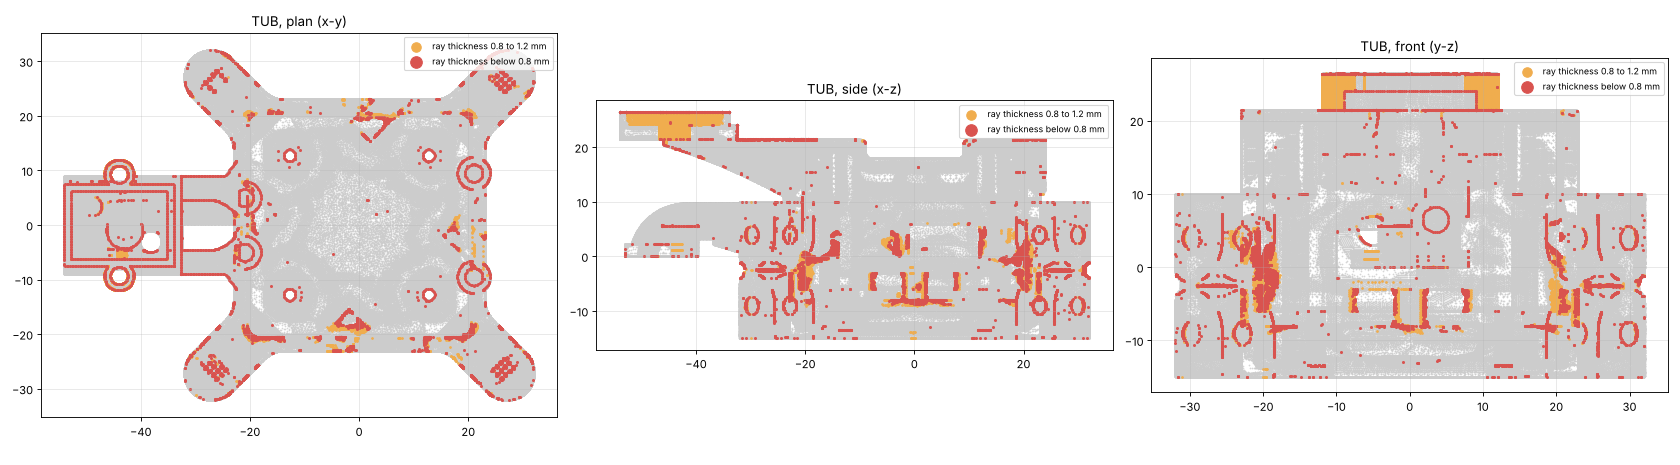
\includegraphics[width=0.9\linewidth]{su_t6_tub_c}
\caption{Wall thickness of the printed tub by the ray method: surface below \SI{0.8}{mm} in red, 0.8 to \SI{1.2}{mm} in yellow.}\label{fig:thickness}
\end{figure}

All parts print in PET-CF with layers in the $xy$ plane. The tub prints on its landing face, where the flight-controller screws enter, which keeps the lid seat on top and lets its flatness be checked with a feeler gauge before assembly.

A fit-test print of the tub, lid and four arms in PLA+ was assembled before the PET-CF parts (\cref{fig:fittest}): the arm forks seat on the tub fins, and the lid closes on the tub rim with the GPS deck behind it.

\begin{figure}[htbp]
\centering
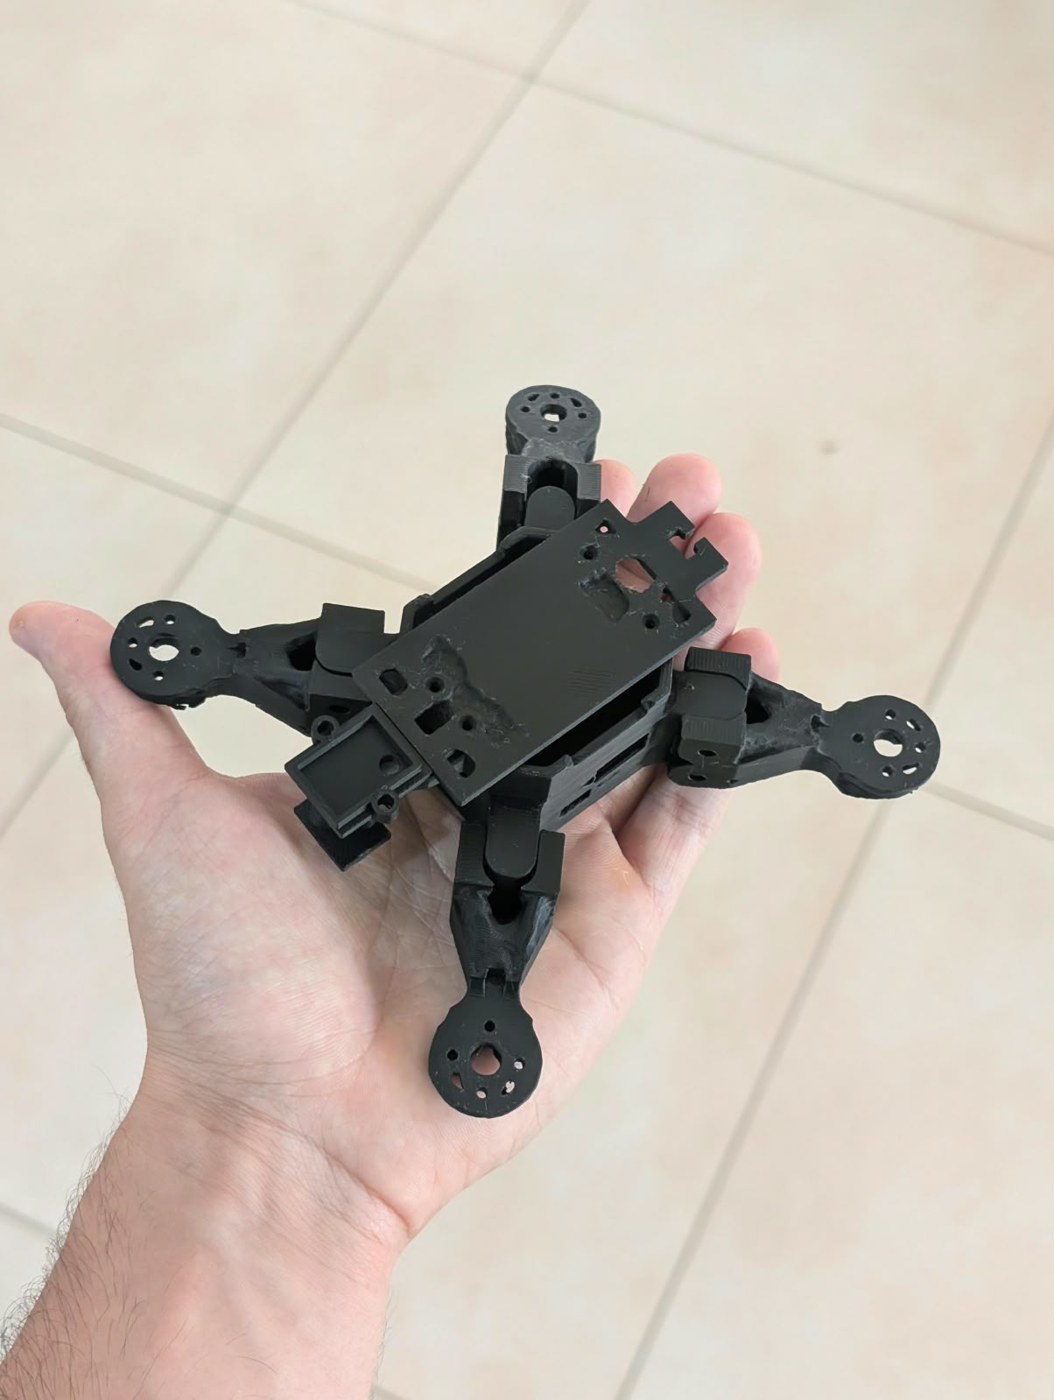
\includegraphics[height=6.4cm]{photo_fit_hand}\hfill
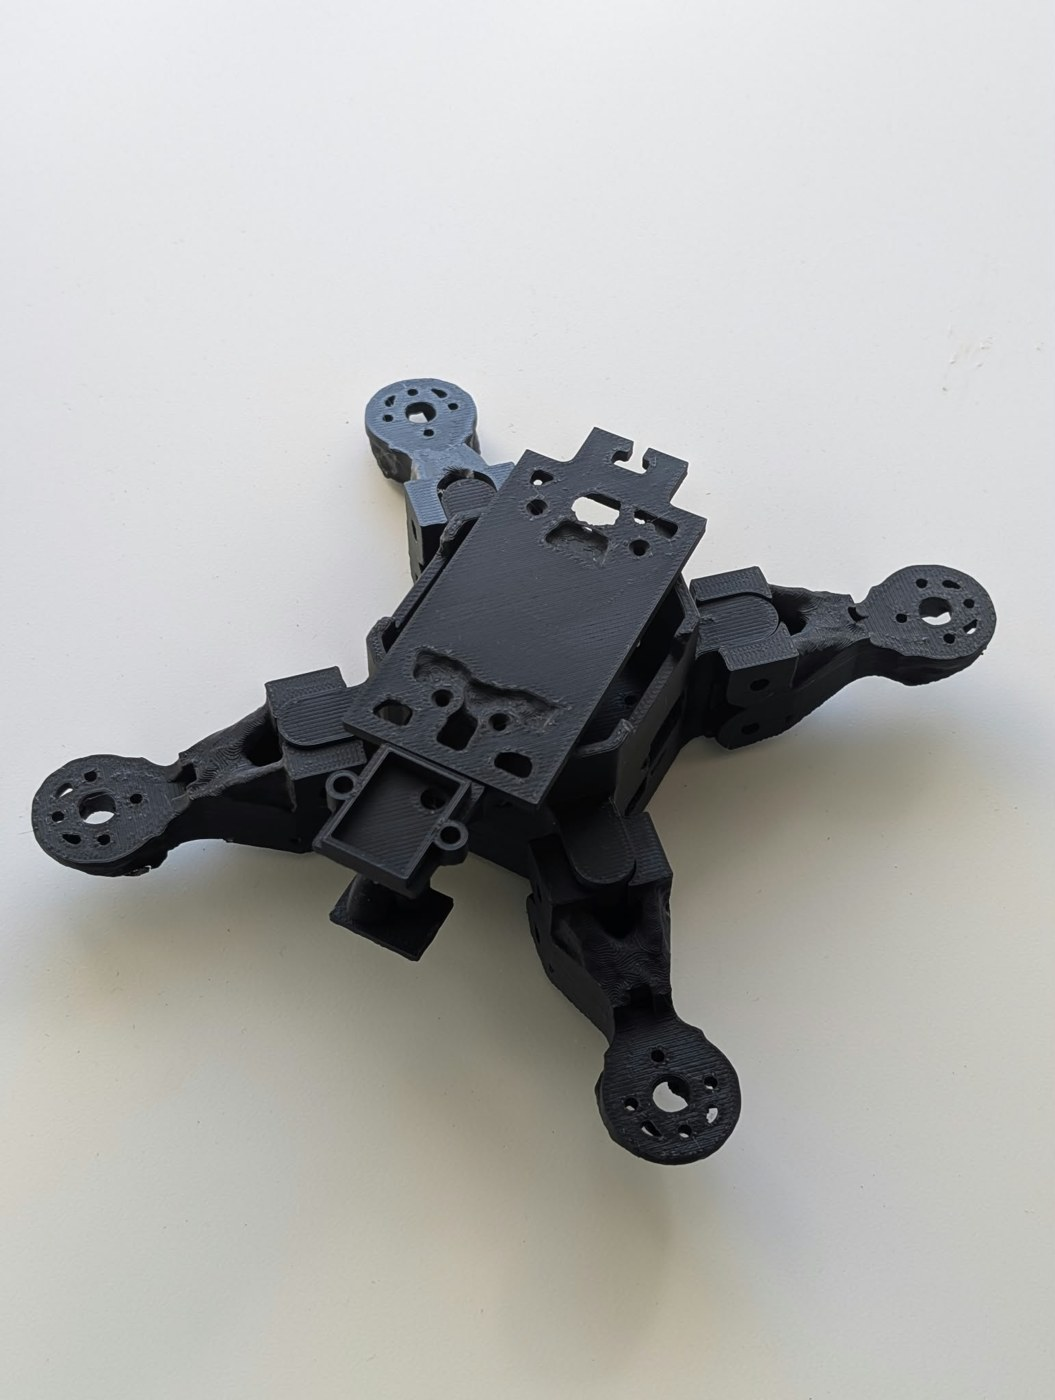
\includegraphics[height=6.4cm]{photo_fit_table}
\caption{Fit-test print of the frame in PLA+: tub, lid and four arms assembled, without components.}\label{fig:fittest}
\end{figure}

\subsection{Retainers}

Components are held by designed seats and three small TPU 95A parts.

\begin{itemize}
\item The receiver cradle (\SI{0.88}{g}) is clamped between the lock nuts and the nylon nuts of two flight-controller screws. The receiver presses in from above past snap lips that overlap its edge by \SI{0.6}{mm}; the antenna connector area stays open for plugging the lead after assembly.
\item The GPS cap (\SI{0.58}{g}) holds the module down with \SI{0.3}{mm} of preload through a \SI{0.8}{mm} plate with a window over the antenna. Two pins of \SI{3.325}{mm} press into the \SI{3.2}{mm} holes of the deck bosses, so the cap needs no screws and no inserts.
\item The antenna holder (\SI{0.94}{g}) clips around both legs of the T antenna with C-clips that wrap \SI{277}{\degree} and is fixed to the keel pad by one M2 screw into a heat-set insert, with a peg for location. The antenna cable bends at a radius of \SI{7}{mm} on its way through the keel, more than six times its diameter.
\end{itemize}

\subsection{Mass and cost}

\begin{table}[htbp]
\centering\small
\caption{Mass of the printed frame and the aircraft.}\label{tab:mass}
\begin{tabular}{@{}lr@{}}
\toprule
Item & Mass\\
\midrule
Tub & \SI{47.21}{g}\\
Lid & \SI{6.61}{g}\\
Four arms & \SI{35.40}{g}\\
\midrule
Frame & \SI{89.22}{g}\\
Components, hardware and retainers (as in the analysis model) & \SI{199.58}{g}\\
\midrule
Take-off mass & about \SI{289}{g}\\
\bottomrule
\end{tabular}
\end{table}

At \SI{40}{EUR/kg} the frame uses about \SI{3.6}{EUR} of filament, against \SI{37.91}{EUR} for the carbon reference frame. The extra \SI{39}{g} of take-off mass above \SI{250}{g} costs about 1.4 minutes of hover time by the mass sensitivity of \cref{sec:sizing}, from 8.2 to about 6.8 minutes.
